\section{Risultati Sperimentali}
\label{sec:risultati}

I dati sperimentali sono stati raccolti utilizzando tre macchine:
\begin{itemize}
    \item Macchina A: ...
    \item Macchina B: ...
    \item \textbf{Macchina C}: \textbf{Intel Core i5-12450H} (12$^\text{a}$ gen, 8 core, 12 thread, fino a 4{,}4~GHz), \textbf{16~GB di RAM DDR4}, SSD \textbf{NVMe PCIe 512~GB} (modello generico \texttt{PCIe-8 SSD 512GB}), sistema operativo \textbf{Arch Linux}, kernel \texttt{6.15.6}, file system \texttt{xfs}.
\end{itemize}

Le macchine erano collegate tramite una rete Ethernet gigabit, con una latenza di circa 0.3 ms.

\subsection{Operazione \texttt{set}}
\label{subsec:risultati-set}

In figura~\ref{fig:bench-set} sono riportati i risultati ottenuti dalle tre macchine durante le operazioni di scrittura.  
I grafici mostrano che le macchine A, B e C hanno raggiunto, rispettivamente, un throughput massimo di $6{,}9 \times 10^3$, $11{,}3 \times 10^3$ e $10{,}3 \times 10^3$ operazioni al secondo.

In figura~\ref{fig:bench-set-all} sono riportati i risultati ottenuti dall'utilizzo congiunto delle tre macchine, con le chiavi distribuite tra di esse senza replicazione.  
Distribuendo le chiavi in modo uniforme, è stato raggiunto un throughput complessivo di $16{,}9 \times 10^3$ operazioni al secondo.  
Utilizzando invece una distribuzione pesata delle chiavi, con pesi pari a $6{:}10{:}10$ tra le macchine, il throughput complessivo è salito a $18{,}8 \times 10^3$ operazioni al secondo, dimostrando l'importanza del meccanismo di allocazione della banda per ottimizzare le performance in scenari distribuiti.  
Sebbene la somma delle capacità individuali teoriche sia pari a $28{,}6 \times 10^3$ operazioni al secondo, il valore effettivamente osservato è inferiore.  
Si osserva inoltre un incremento della latenza rispetto all'esecuzione su una singola macchina. Tuttavia, a differenza dei test su macchina singola, la latenza rimane pressoché costante all'aumentare della frequenza delle operazioni.  
Si ipotizza che tali effetti siano attribuibili all'overhead introdotto dalla comunicazione e dal coordinamento tra nodi distribuiti.

\begin{figure}[htbp]
    \centering
    \begin{minipage}[t]{0.48\textwidth}
        \centering
        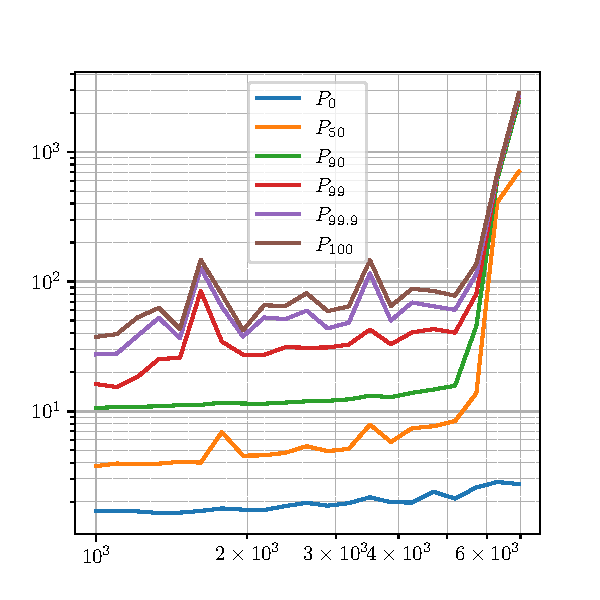
\includegraphics[width=\textwidth]{03-risultati/freq-latency/bench-set-a}
        \caption*{Macchina A}
    \end{minipage}
    \hfill
    \begin{minipage}[t]{0.48\textwidth}
        \centering
        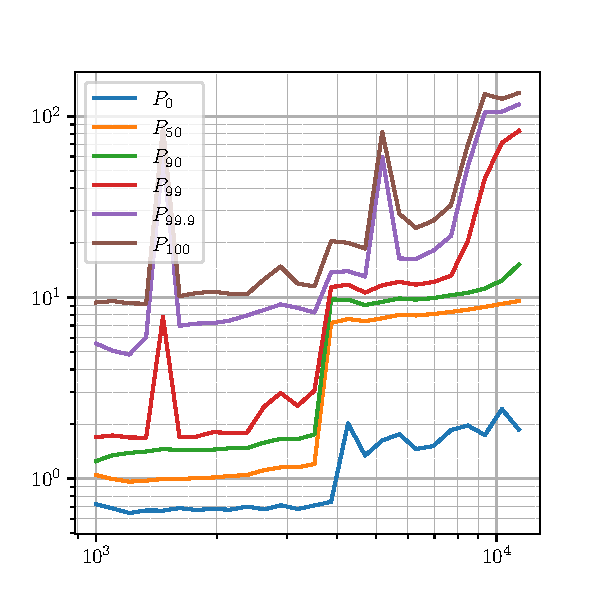
\includegraphics[width=\textwidth]{03-risultati/freq-latency/bench-set-c}
        \caption*{Macchina B}
    \end{minipage}

    \vspace{0.5cm}
    \begin{minipage}[t]{0.48\textwidth}
        \centering
        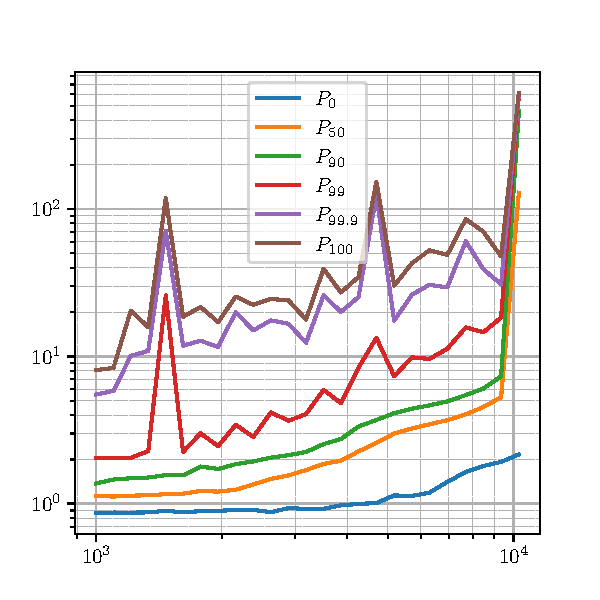
\includegraphics[width=\textwidth]{03-risultati/freq-latency/bench-set-h}
        \caption*{Macchina C}
    \end{minipage}

    \caption{Performance delle macchine in scrittura. Ogni grafico rappresenta, al variare della frequenza delle operazioni [Hz], la latenza [ms] osservata per diversi percentili (dal P0 al P100).}
    \label{fig:bench-set}
\end{figure}

\begin{figure}[htbp]
    \centering
    \begin{minipage}[t]{0.48\textwidth}
        \centering
        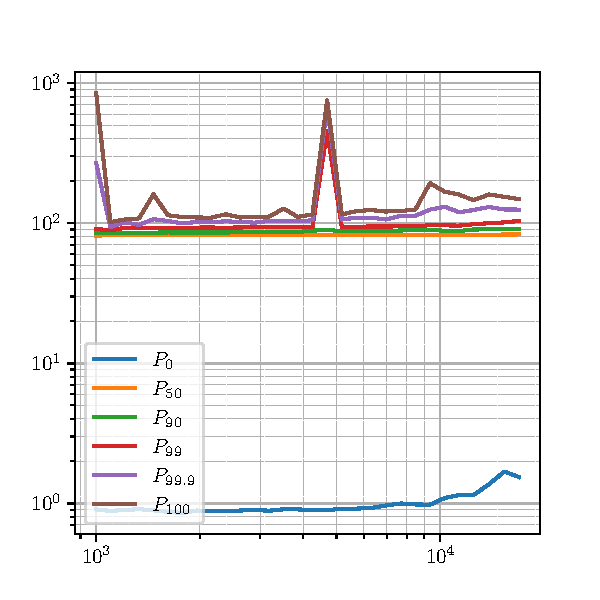
\includegraphics[width=\textwidth]{03-risultati/freq-latency/bench-set-all}
        \caption*{Chiavi distribuite uniformemente sulle tre macchine}
    \end{minipage}
    \hfill
    \begin{minipage}[t]{0.48\textwidth}
        \centering
        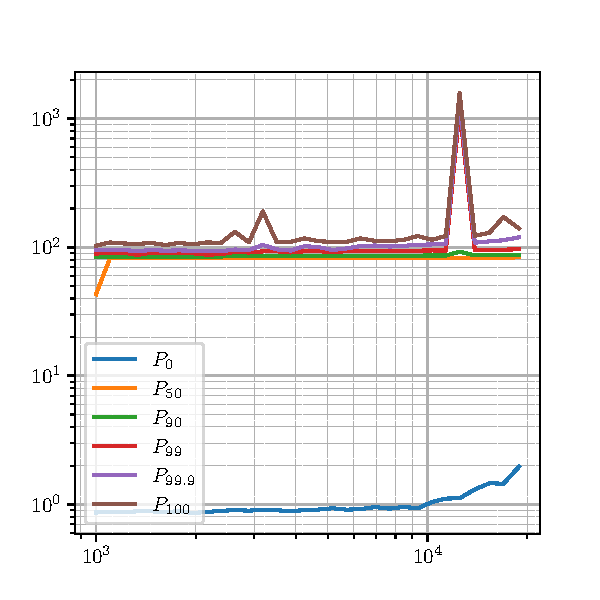
\includegraphics[width=\textwidth]{03-risultati/freq-latency/bench-set-all-balance}
        \caption*{Chiavi distribuite sulle tre macchine con pesi bilanciati [6:10:10]}
    \end{minipage}

    \caption{Performance delle macchine in scrittura distribuita. Ogni grafico rappresenta, al variare della frequenza delle operazioni [Hz], la latenza [ms] osservata per diversi percentili (dal P0 al P100).}
    \label{fig:bench-set-all}
\end{figure}

\subsection{Operazione \texttt{get}}
\label{subsec:risultati-get}

In figura~\ref{fig:bench-get} sono riportati i risultati ottenuti dalle tre macchine durante le operazioni di lettura.  
I grafici mostrano che le macchine A, B e C hanno raggiunto, rispettivamente, un throughput massimo di $25{,}6 \times 10^3$, $45{,}4 \times 10^3$ e $50{,}0 \times 10^3$ operazioni al secondo. In utilizzo congiunto, le tre macchine hanno raggiunto un throughput complessivo di $20{,}8 \times 10^3$ operazioni al secondo.
A causa della cache del sistema operativo sul file system, il costo della comunicazione tra le macchine risulta maggiore rispetto al costo dell'operazione di lettura stessa, causando un peggioramento delle performance rispetto all'esecuzione su una singola macchina.  
Si ipotizza che, utilizzando un database di dimensioni maggiori rispetto alla RAM disponibile, la situazione possa invertirsi. Tuttavia, non è stato possibile testare direttamente questa ipotesi.

\begin{figure}[htbp]
    \centering
    \begin{minipage}[t]{0.48\textwidth}
        \centering
        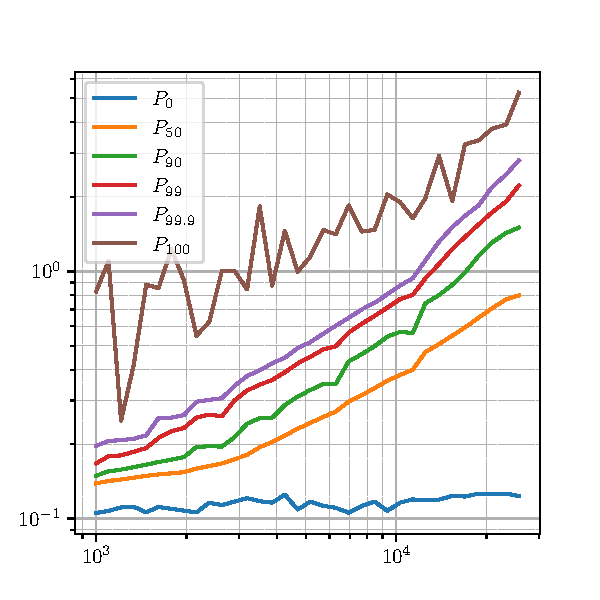
\includegraphics[width=\textwidth]{03-risultati/freq-latency/bench-get-a}
        \caption*{Macchina A}
    \end{minipage}
    \hfill
    \begin{minipage}[t]{0.48\textwidth}
        \centering
        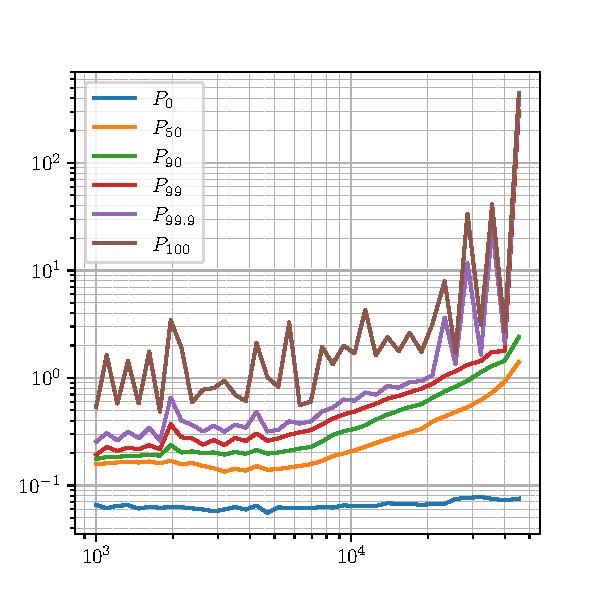
\includegraphics[width=\textwidth]{03-risultati/freq-latency/bench-get-c}
        \caption*{Macchina B}
    \end{minipage}

    \vspace{0.5cm}
    \begin{minipage}[t]{0.48\textwidth}
        \centering
        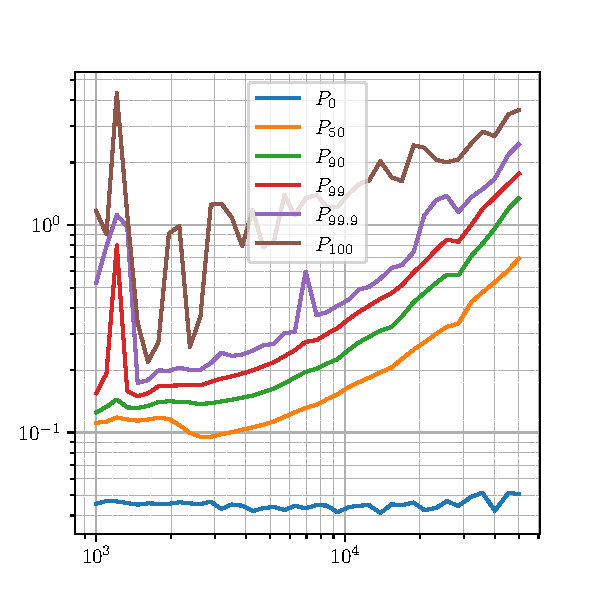
\includegraphics[width=\textwidth]{03-risultati/freq-latency/bench-get-h}
        \caption*{Macchina C}
    \end{minipage}
    \hfill
    \begin{minipage}[t]{0.48\textwidth}
        \centering
        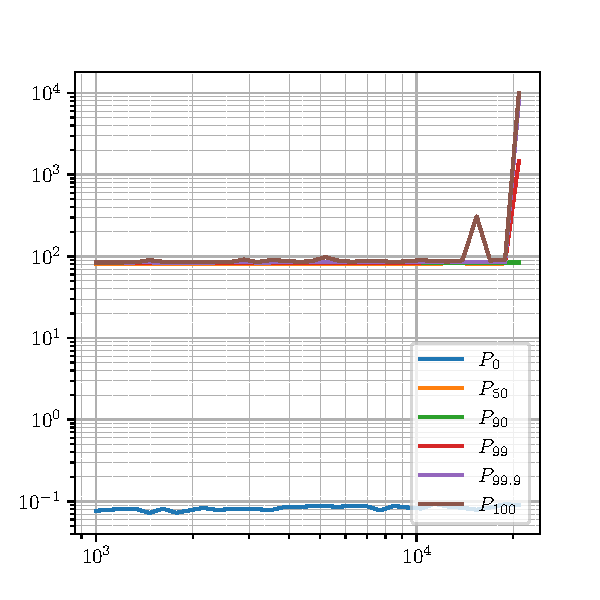
\includegraphics[width=\textwidth]{03-risultati/freq-latency/bench-get-all}
        \caption*{Chiavi distribuite uniformemente sulle tre macchine}
    \end{minipage}

    \caption{Performance delle macchine in lettura. Ogni grafico rappresenta, al variare della frequenza delle operazioni [Hz], la latenza [ms] osservata per diversi percentili (dal P0 al P100).}
    \label{fig:bench-get}
\end{figure}

\subsection{Dimesione dei Valori}
\label{subsec:risultati-dimensione}

TODO

\subsection{Multitenant}
\label{subsec:risultati-multitenant}

TODO
